\begin{figure}[h]
	\centering
	\begin{subfigure}[b]{0.3\textwidth}
		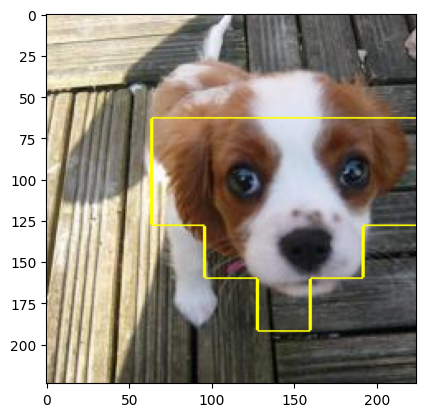
\includegraphics[width=.9\textwidth]{img/examples/appendix/n02086646_12074_gradcam}
		\caption{GradCAM IoU=0.439218}
	\end{subfigure}
	\begin{subfigure}[b]{0.3\textwidth}
		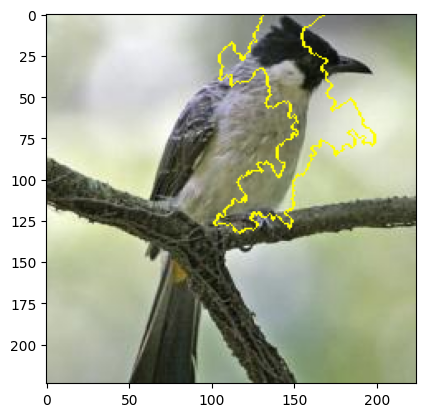
\includegraphics[width=.9\textwidth]{img/examples/appendix/n01560419_47474_lime}
		\caption{LIME IoU=0.176749}
	\end{subfigure}
	\begin{subfigure}[b]{0.3\textwidth}
		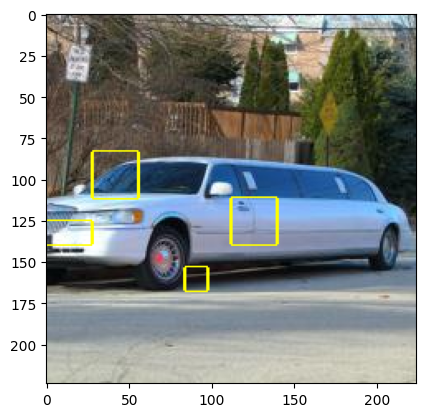
\includegraphics[width=.9\textwidth]{img/examples/appendix/n03670208_41512_shap}
		\caption{SHAP IoU=0.118568}
	\end{subfigure}
	\caption{Przykłady wyjaśnień dla których IoU jest bliskie ich średniej}
	\label{}
\end{figure}

\begin{figure}[h]
	\centering
	\begin{subfigure}[b]{0.3\textwidth}
		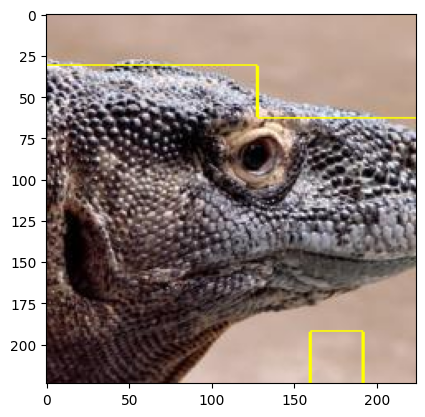
\includegraphics[width=.9\textwidth]{img/examples/appendix/n01695060_35102_gradcam}
		\caption{GradCAM IoU=0.988630}
	\end{subfigure}
	\begin{subfigure}[b]{0.3\textwidth}
		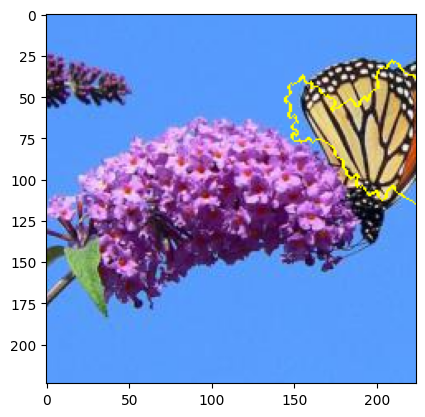
\includegraphics[width=.9\textwidth]{img/examples/appendix/n02279972_47456_lime}
		\caption{LIME IoU=0.619109}
	\end{subfigure}
	\begin{subfigure}[b]{0.3\textwidth}
		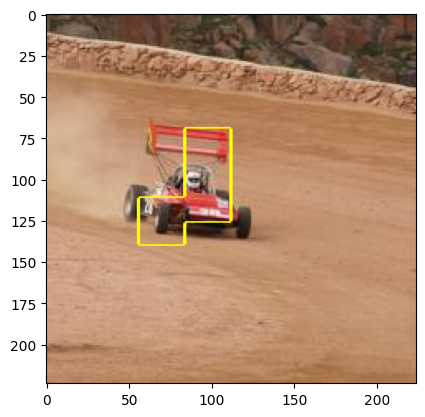
\includegraphics[width=.9\textwidth]{img/examples/appendix/n04037443_42773_shap}
		\caption{SHAP IoU=0.486928}
	\end{subfigure}
	\caption{Przykłady wyjaśnień dla których IoU jest większe niż normalnie}
\end{figure}
